\documentclass{article}
\usepackage{graphicx} % Required for inserting images
\usepackage{amsfonts}

\title{24.08.27 Settings of MuSig, Mithril and Lookup Argument}
\author{Xun Zhang \quad \quad Wuyun Siqin \quad \quad Bingsheng Zhang \\ 
Zhejiang University, CHN \\
22221024@zju.edu.cn \quad 3210101763@zju.edu.cn \quad bingsheng@zju.edu.cn}

\date{August 27 2024}

\begin{document}

\maketitle

\section{Aggregator Node}

We first introduce the setting of aggregator node in MuSig2 [NRS21]. And it is necessary to clarify the syntax of the two-round multi-signature scheme. The following contents is from original paper.
\\
\\
It consists of algorithms

\[
\mathsf{(Setup,KeyGen,KeyAgg,(Sign, SignAgg, Sign', SignAgg', Sign''), Ver)}
\]

as follows. System-wide parameters $par$ are generated by the setup algorithm Setup taking as input the security parameter. For notational simplicity, we assume that $par$ is given as implicit input to all other algorithms. The randomized key generation algorithm takes no input and returns a secret/public key pair $(sk, pk) \leftarrow \mathsf{KeyGen()}$.
The deterministic key aggregation algorithm $\mathsf{KeyAgg}$ takes a multiset of public keys $L = \{pk_1,...,pk_n\}$ and returns an aggregate public key: $\tilde pk = \mathsf{KeyAgg}(\{pk_1,...,pk_n\})$.
The interactive signature algorithm $\mathsf{(Sign, SignAgg, Sign', SignAgg', Sign')} $is run by each signer $i$ and proceeds in a sequence of two communication rounds.

For instance, from the point of view of signer 1, a full signing run proceeds as follows:
\[
(out_1, state_1) \leftarrow \mathsf{Sign()}
\]
\[
 out := \mathsf{SignAgg}(out_1, . . . , out_n)
\]
\[
(out_1', state_1') \leftarrow \mathsf{Sign'}(state_1, out, sk_1, m, \{pk_2,...,pk_n\})
\]
\[
out':= \mathsf{SignAgg'}(out_1', . . . , out_n')
\]
\[
\sigma \leftarrow \mathsf{Sign''}(state_1', out')
\]
The purpose of the aggregation algorithms $\mathsf{SignAgg}$ and $\mathsf{SignAgg'}$ is to enable savings in the broadcast communication in both signing rounds: An aggregator node [SS01; KG20], which will be
untrusted in our security model and can for instance be one of the signers, can collect the outputs of all signers in both rounds, aggregate the outputs using $\mathsf{SignAgg}$ and $\mathsf{SignAgg'}$, respectively, and broadcast only the aggregate output back to all signers. This optimization is entirely optional. If it is not desired, each signer can simply broadcast its outputs directly to all signers, which then all run $\mathsf{SignAgg}$ and $\mathsf{SignAgg'}$ by themselves.




\section{Mapping in Mithril}

In Mithril, the relation we need to prove includes:

\begin{itemize}
    \item For $i = 1..k: \mathsf{MSP.Eval}(msg, \mathsf{index}_i, \sigma_i) = ev_i$
    \item For $i = 1..k: ev_i \leq \phi(\mathsf{stake}_i)$
\end{itemize}

There are two constructions of mapping: one is based on Bulletproofs and the other based on releasing the witness. 

The Bulletproofs construction uses Elligator Squared, which avoids oracle calls on user-specific data i.e. we explicitly avoid hashing $\sigma$ to sidestep soundness issues in circuit-based proofs.

For the concatenation proof system(the one just releases the witness), use a random oracle $H : {0, 1}* \rightarrow \mathbb{Z}_p$ to implement the mapping as: $M^R_{msg,index}(\sigma) := H("map"||msg||\mathsf{index}||\sigma)$.

In Mithril official code, they use Blake2b hash function to map the information:

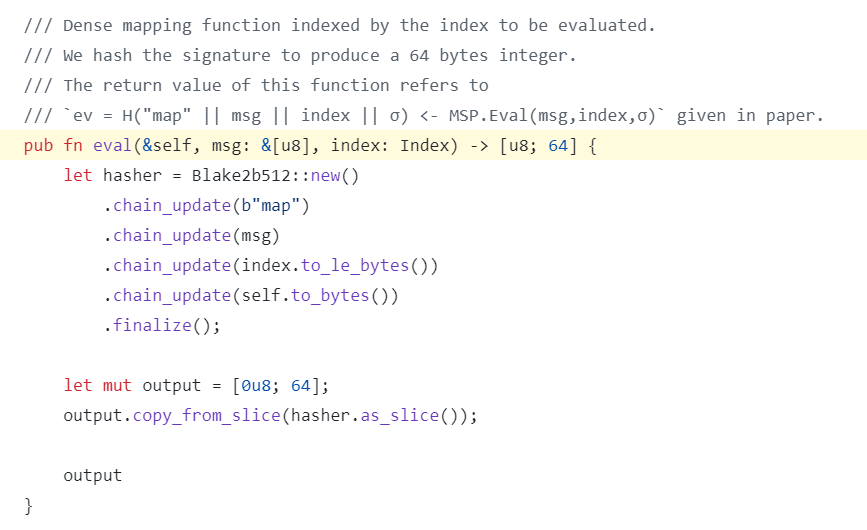
\includegraphics[width=1\linewidth]{mithril-mapping-code.png}

And this value will be checked in the $\phi$ funtion:

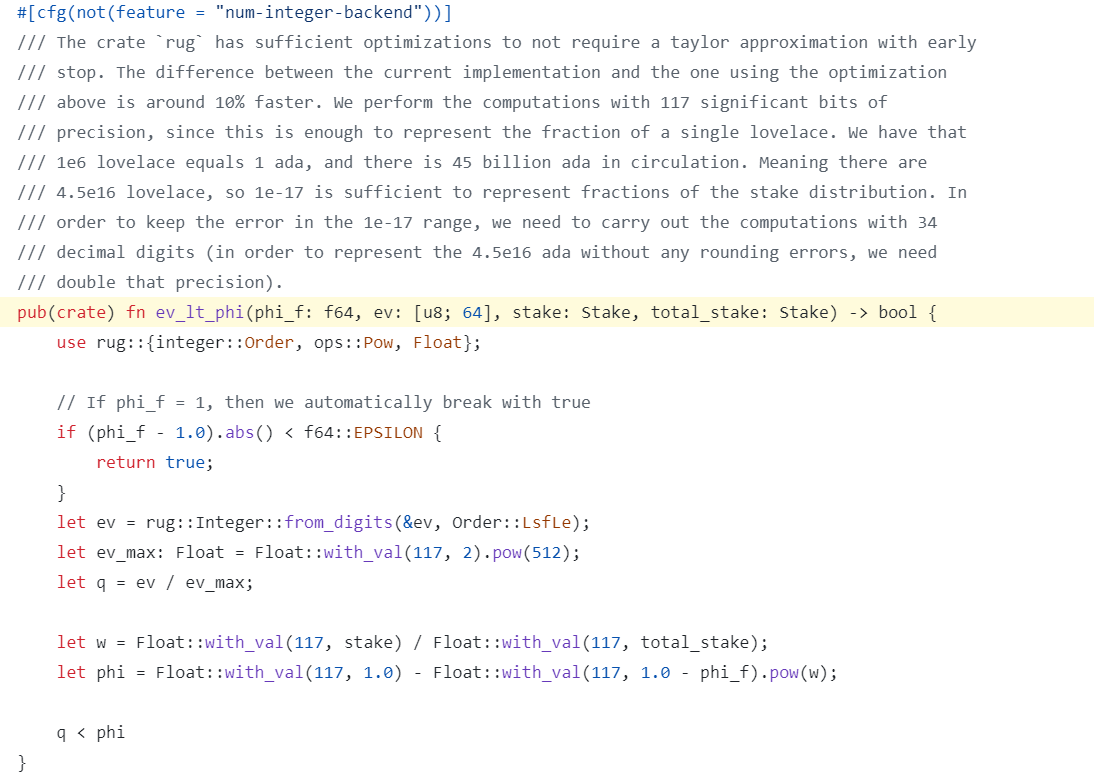
\includegraphics[width=1\linewidth]{mithril-phi-code.png}


So if we choose to write a circuit of Blake2b hash function, it will be heavy. Or we replace the Blake2b with Poseidon hash function, just as we did in merkle tree.

So now let's estimate the number of constraints. Assume there are $k$ valid signers, each one will produce a valid BLS signature, and each signer offers a won lottery index.
The cost will be:
\begin{itemize}
    \item $k$ Rescue hash functions for $e_v$. Since we use merkle tree with rate = 3, it will be $2k$ Rescue permuitation.
    \item $k$ $\phi$ function evaluations.
    \item $k$ Comparisons between $e_v$ and $\phi(stake)$.
\end{itemize} 
The actual constraints number needs further evaluation.

If we choose the approach in original paper, the cost will be:

\begin{itemize}
    \item $k$ Mapping evaluations for $e_v$(use Elligator Squared).
    \item $k$ $\phi$ function evaluations.
    \item $k$ Comparisons between $e_v$ and $\phi(stake)$.
\end{itemize}

And the paper also give the constraints number:
\begin{itemize}
    \item $3k\log q + 60k$ for representation function evaluations.
\end{itemize}

Because Mapping representations involve 60 constraints plus 3 range checks. One is for comparison between $e_v$ and $\phi(stake)$ and other two for range checks for index.

And there is also a optimization for $\phi(stake)$, you can see that there is no constraints for $\phi$ evaluation. The following contents is from Mithril paper:
\\

\textit{The main outlier is the evaluation of $\phi$. Fortunately, we don’t actually need to evaluate $\phi$ in the proof: we can replace stake in the tree with $\phi(stake)$ and proceed with the comparison directly. This gives us a circuit size of $O(klogq)$, and verifier complexity of $O(\frac{klog^4q}{log(klogq)})$ as verification is dominated by a multiexponentiation based on the circuit size.}


\section{SNARK-based Mithril Implementation}

We met a problem when implementing the following relations:

\begin{enumerate}
    \item $ivk=\prod mvk_i^{e_i} $, where $e_i \leftarrow \textrm{H}(i,e_\sigma)$.
    \item $\mu \leftarrow \prod \sigma_i^{e_i}$, where $e_i \leftarrow \textrm{H}(i,e_\sigma)$ and $e_\sigma \leftarrow \textrm{H}(\mathbb{\sigma})$.
\end{enumerate}

We firstly compute the weighting seed $e_\sigma$ and the coefficient $e_i$ according to the indices:
\\
\\
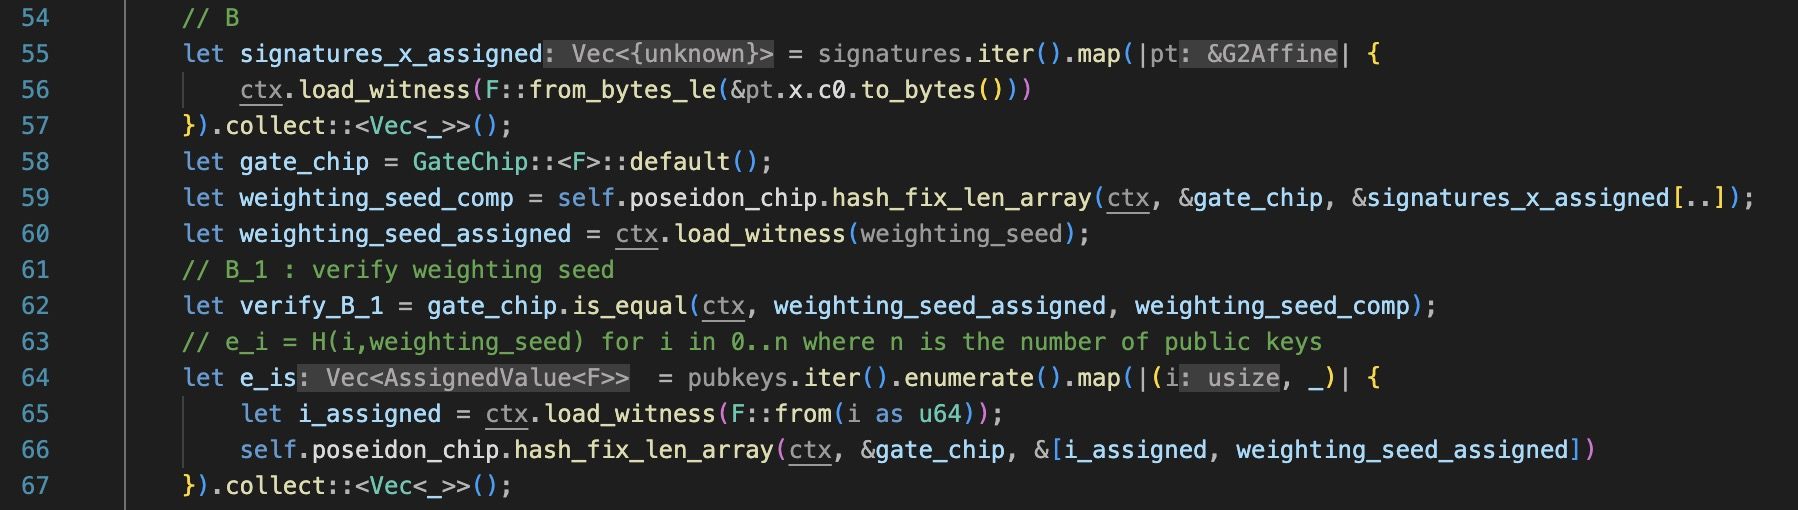
\includegraphics[width=1\linewidth]{halo2-lib-ei.jpg}


And use the $e_i$ coefficient to combine all the public keys and signatures:
\\
\\
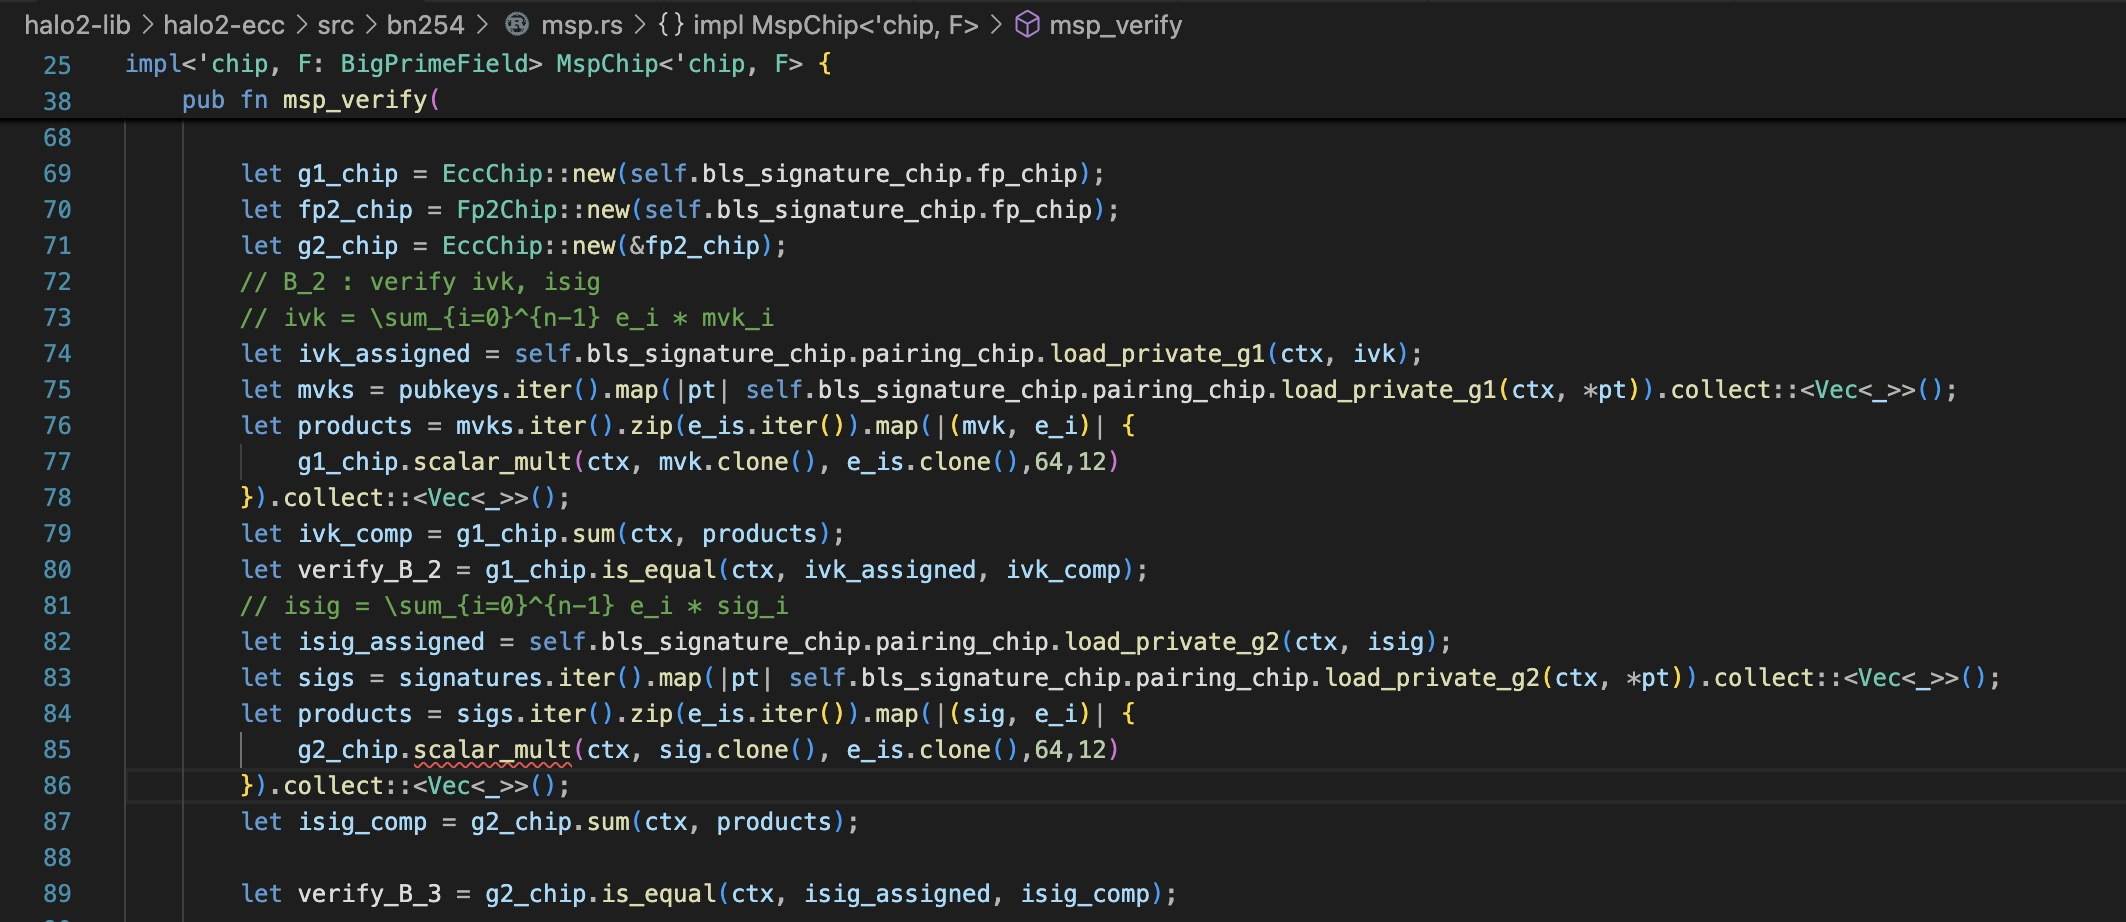
\includegraphics[width=1\linewidth]{halo2-lib-Bsig-wrong.jpg}

There is an error when we try to make a scalar multiplication between $\sigma$ and coefficient $e_i$. Maybe it's because $e_i$ is a $\mathbb{G}_1$ scalar value, and it cannot be multiplied by a $\mathbb{G}_2$ element directly. It is a problem remains to be solved.


\section{Shuffle Argument}

% \subsection{}
The public keys(\textbf{pk}) we use are points on an elliptic curve. We can compress a point on the elliptic curve.

For any finite point \( P = (x_P, y_P) \) on the elliptic curve, this point can be succinctly represented by storing only the \( x \)-coordinate \( x_P \) and a specific bit derived from \( x_P \) and \( y_P \), known as the compressed representation of the point.

Specifically, let \( P = (x_P, y_P) \) be a point on the elliptic curve \( E: y^2 = x^3 + ax + b \) defined over \( \mathbb{F}_p \). If \( y_{rb} \) is the rightmost bit of \( y_P \), then the point \( P \) can be represented by \( x_P \) and \( y_{rb} \).

According to our previous approach, for shuffling \textbf{pk} , we used the following strategy. A compressed representation of a \textbf{pk} in the set is denoted as \( (pk_x, pk_{yb}) \). We treat the vector \( PK' \) as a shuffle of the vector \( PK \), introducing two challenge values \( \gamma \) and \( \zeta \). We compute:

\begin{enumerate}
    \item \( \prod_{i=1}^{n} (pk_x + \gamma \cdot pk_{yb} + \zeta) \).
    \item \( \prod_{i=1}^{n} (pk_x' + \gamma \cdot pk_{yb}' + \zeta) \).
\end{enumerate}

If the following equality holds:
\[
\prod_{i=1}^{n} (pk_x + \gamma \cdot pk_{yb} + \zeta) = \prod_{i=1}^{n} (pk_x' + \gamma \cdot pk_{yb}' + \zeta)
\]

then \( PK' \) is a permutation of \( PK \).

\subsection{Cost Discussion for Different Scheme Combinations}

Consider a set of \( N \) elements in the PK collection, from which we select \( m \) elements for signature aggregation:

When we use Merkle path for verification, the cost is \( O(m \log N) \).

When we use shuffle arguments for verification, the cost is \( O(N) \). The cost for proving the Merkle root of the PK set is \( 2N \), so the total cost is \( O(N) \).

In this context, if \( m \) is linear in \( N \), then the cost of the second scheme is smaller. However, if \( m \) is sub-linear or smaller, then the cost of the first scheme is lower.

% \section{Future Direction}
% Merkle path do not need to read all the pks, but shuffle arguement do.




% \section{Subset Argument/Lookup Argument}
% Halo2 expresses lookups in terms of a "subset argument" over a table with \(2^k\) rows (numbered from 0) and columns \(A\) and \(S\). 

% The goal of the subset argument is to enforce that every cell in \(A\) is equal to some cell in \(S\). This means that more than one cell in \(A\) can be equal to the same cell in \(S\), and some cells in \(S\) don't need to be equal to any of the cells in \(A\).







\end{document}

